\chapter{Dynamic Programming}

\section{Longest Increasing Subsequence}

    If needed, the algorithm for LIS can be easily modified for 
    the similar task of \textbf{Longest Non-Decreasing Subsequence}.

    \kactlimport{lis.cpp}

\section{Divide-Conquer Optimization}

        Some dynamic programming problems have a recurrence of this form:

        $$ dp[i][k] = \min_{1 \leq j \leq i} dp[j - 1][k - 1] + C(j, i) $$

        Where $dp[i][k] $ is the \textit{min cost} considering the element up to $i$ with exactly $k$ partitions.

        Additionally, $C(j, i)$ is the cost of the partition $[j, i]$ and $dp[i][k] = 0$ when $k = 0$.

        Say $ 1 \leq i \leq n $ (1-idx) and $1 \leq k \leq m$, and evaluating $C$ takes $O(1)$ time. 
        Then the straightforward evaluation of the above recurrence is $O(m n^2)$. There are
        $n \times m$ states, and $n$ transitions for each state.

        Let $opt(i, k)$ be the value of $j$ that minimizes the above expression, $opt(i, k)$ is the optimal splitting point.

        Assuming that the cost function satisfies the \textit{quadrangle inequality} (``wider is worse''), we can show that
        $opt(i-1, k) \leq opt(i, k)$ for all ${i, k}$. This is known as the \textit{monotonicity condition}. In other words,
        for a fixed $k$, the optimal splitting point $opt(i, k)$ increases as $i$ increases.

        This lets us solve for all states more efficiently. Say we computed $opt(i, k)$ for some fixed $i$ and $k$. 
        Then, for any $i' < i$, we know that $opt(i', k) \leq opt(i, k)$. 
        This means when computing $opt(i', k)$, we don't have to consider as many splitting points!

        To minimize the runtime, we use this property and apply the idea behind \textit{divide and conquer} 
        and call the functions to solve recursively. Compute the $opt(l, mid)$ and using this value, 
        solve $opt(l, mid-1)$ and $opt(mid+1, r)$.
        
        By recursively keeping track of the lower and upper bounds on $opt$, 
        we reach a $O(n \log n)$ runtime per $k$. Each possible value of $opt(i, k)$ only appears in $\log n$ different nodes.

        \textbf{Problems that can be solved:}

        \begin{itemize}
        \item \textbf{Subarray Squares}: \textit{cost} = square of the sum in each partition.
        \item \textbf{Houses and Schools}: each partition has a school at the \textit{right endpoint}, 
        and the cost is the accumulated walking time for each house, split in the middle, each half walking to the closest school.
        Precomputed $dp[i][1]$ considers the left border only walking right. Finally, $ans$ is computed with $dp[i][m]$ + walking left of the remaining right border.
        \end{itemize}

        \kactlimport{divide-conquer-dp.cpp}

\section{Knuth Optimization}

    Knuth's optimization, also known as the Knuth-Yao Speedup, is a special case of dynamic programming on ranges, 
    that can optimize the time complexity of solutions by a linear factor, from $O(n^3)$ for standard range DP to $O(n^2)$.

    \subsection{Conditions}

        The Speedup is applied for transitions of the form:

        $$dp(i, j) = \min_{i \leq k < j} [ dp(i, k) + dp(k+1, j) + C(i, j) ].$$

        Similar to divide and conquer DP, let $opt(i, j)$ be the value of $k$ that minimizes the expression in the transition 
        ($opt$ is referred to as the "optimal splitting point" further in this article). The optimization requires that the following holds:

        $$opt(i, j-1) \leq opt(i, j) \leq opt(i+1, j).$$

        We can show that it is true when the cost function 
        $C$ satisfies the following conditions for $a \leq b \leq c \leq d$:

        $C(b, c) \leq C(a, d)$;

        $C(a, c) + C(b, d) \leq C(a, d) + C(b, c)$ (the quadrangle inequality [QI]).

        A common cost function that satisfies the above condition is the \textbf{sum of the values in a subarray}.

        \kactlimport{knuth.cpp}

\section{Slope Optimizations}

    \subsection{Convex Hull Trick}

        If multiple transitions of the DP can be seen as 
        first degree polynomials (lines). CHT can be used to optimized it

        Some valid functions:

        $ax + b$
        
        $cx^2 + ax + b$ 
        (ignore $cx^2$ if c is independent)

        \kactlimport{cht-dynamic.cpp}

    \subsection{Li-chao Tree}

        Works for any type of function that has the \textbf{transcending property}:

        Given two functions $f(x)$, $g(x)$ of that type, 
        if $f(t)$ is greater than/smaller than $g(t)$ for some $x=t$,
        then $f(x)$ will be greater than/smaller than $g(x)$ for $x>t$.
        In other words, once $f(x)$ “win/lose” $g(x)$, $f(x)$ will continue to “win/lose” $g(x)$.

        The most common one is the line function: $ax + b$

        Due to the segment tree structure, Li-Chao tree also supports adding line \textbf{segments}.

        \kactlimport{lichao.cpp}
        
        \kactlimport{li-chao-sparse.cpp}

    % for notebook generation
    \vspace{5pts}

    \subsection{Slope Trick}
    
    You are given an array of n integers. You want to modify the array so that it is non-decreasing, i.e., every element is at least as large as the previous element.
    On each move, you can increase or decrease the value of any element by one. What is the minimum number of moves required?
    
    \textbf{Observation: } It is also possible to solve the problem of modifying the array to stricly increasing.

    \kactlimport{slope-trick.cpp}

\section{SOS DP}

    \textbf{Sum over Subsets DP (SOS DP)} computes how many elements there are for each mask
    which are a subset of this mask.

    This can be modified for other operations in which the subset contributes for the mask
    .
    \textit{Example:}

    \textbf{10}0\textbf{1} if a subset of \textbf{11}0\textbf{1};

    \textbf{00}0\textbf{1} if a subset of \textbf{11}0\textbf{1};
    
    \textbf{11}0\textbf{0} if a subset of \textbf{11}0\textbf{1};
    
    \textbf{11}0\textbf{1} if a subset of \textbf{11}0\textbf{1};

    \begin{center}
        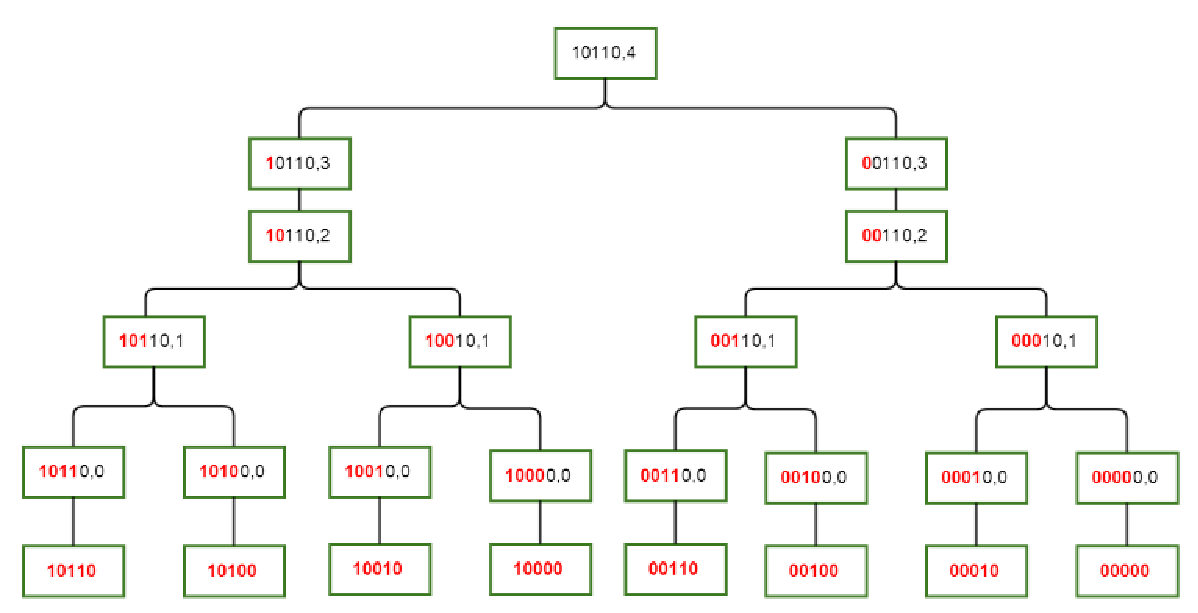
\includegraphics[width=9cm]{content/dynamic-programming/sos-example.pdf}
    \end{center}

    \kactlimport{sos-dp.cpp}

\section{Bit optimization}

    \textbf{use popcnt pragma!!}

    \begin{lstlisting}[language=c++]
    #pragma GCC target("popcnt")
    \end{lstlisting}

    \subsection{Operations}

    \begin{align*}
        intersection & \hspace{5mm} & a \cap b     & \hspace{5mm} &  a \& b \\
        union        & \hspace{5mm} & a  \cup b    & \hspace{5mm} &  a | b \\
        complement   & \hspace{5mm} & \overline{a} & \hspace{5mm} &  ~a \\
        difference   & \hspace{5mm} & a - b        & \hspace{5mm} &  a \& (~b) \\
    \end{align*}

    \begin{itemize} 
        \item \textbf{\_\_builtin\_clz(x)}: the number of zeros at the beginning of the number
        \item \textbf{\_\_builtin\_ctz(x)}: the number of zeros at the end of the number
        \item \textbf{\_\_builtin\_popcount(x)}: the number of ones in the number
        \item \textbf{\_\_builtin\_parity(x)}: the parity (even or odd) of the number of ones

        \item \textbf{LSB(i)}: ((i) \& -(i))
        \item \textbf{MSB(i)}: (63 - \_\_builtin\_clzll(i)), for ll
    \end{itemize}
    
    \subsection{Bitset}

    Bitset are very convenient for bitwise operations. Beside common operators, there are other useful ones already built in:
    
    \begin{itemize} 
        \item \textbf{bitset $<$k$>$ bs(str)}: create a bitset of size k from a binary string representation
        \item \textbf{bitset $<$k$>$ bs(num)}: create a bitset of size k from a integer representation
        \item \textbf{str = bs.to\_string()}: return the binary string representation of the bitset
        \item \textbf{num = bs.to\_ullong()()}: return the unsigned integer representation of the bitset
        \item \textbf{bs.\_Find\_first()}: returns the first set bit (from LSB to MSB)
        \item \textbf{bs.\_Find\_next(idx)}: returns the next set bit after idx (not including idx of course)
    \end{itemize}

    Note that, if there isn't any set bit after idx, BS.\_Find\_next(idx) will return BS.size(); 
    same as calling BS.\_Find\_first() when bitset is clear;
    One can use \textbf{bs.\_Find\_next(idx-1)} to include idx. The function does accept negative index. 

    The complexity of bitwise operations for the bitset is $O(\frac{size}{32})$ or $O(\frac{size}{64})$, 
    depending on the architecture of the computer.
    
    \subsection{Problems}
    
    \begin{itemize}
        \item \textbf{Hamming Distance:} When comparing two binary strings of size $k$, if the size of the strings are small enough, 
        just represent them as integers (uint or ulong) and do \textit{\_\_builtin\_popcount(a \^ b)} to compute the hamming distance in $O(1)$ instead of $O(k)$.

        \item \textbf{Counting subgrids:} If the desired size if not small enough, divide into continuous segments of acceptable sizes (such as k=64 for unsigned long long).
        Then, the complexity of $O(N)$ can be reduced to $O(N/64)$. 
        For more versatility, and huge sizes, one can use $bitset<k>$ directly, but it is a little bit slower.

    \end{itemize}

\section{Knapsacks}

Given the costs $c_i$ and values $v_i$ of $N$ items, put these items in a knapsack of capacity $W$ 
to get the maximum total value in the knapsack.

%notebook
\vspace{4pts}

\subsection{Fractional Knapsack}

    In Fractional Knapsack, we can break items for maximizing the total value of the knapsack.

    \textbf{Solution:} Greedly use the best items (bigger $\frac{v_i}{c_i}$ ratios).

%notebook
\vspace{4pts}

\subsection{0/1 Knapsack}

    Traditional Knapsack.

    \textbf{Solution:} $O(N W)$ dp solution.

    \kactlimport{knapsack-01.cpp}

%notebook
\vspace{4pts}

\subsection{Bounded Knapsack}

    In Bounded Knapsack, in addition to $c_i$ and $v_i$, each item has a max quantity available $q_i$.
    
    \textbf{Solution:} $O(N W \log{max(Q)})$ dp solution. Break each item into binary partitions.
    
    \textit{Example:} Given a item with $q = 11$, break it into $3$ different items: 
    $q_1 = 1$, $q_2 = 2$, $q_3 = 8$

\subsection{0/1 Knapsack with limited summation}

    This Knapsack, has a additional constrain saying that $\sum{c_i} \leq N$.

    Because of this, we can conclude that, in the worst case, there will be only $O(\sqrt(N))$ unique items.

    Simply create a histogram of the items and convert this problem to a bounded knapsack problem.

    \textbf{Solution:} $O(\sqrt{N} W \log{max(Q)})$ dp solution.
